\documentclass{article}
\usepackage{graphicx} % Required for inserting images
\usepackage{amsfonts}
\usepackage[T1]{fontenc}
\usepackage{comment}
\usepackage{emoji}
\usepackage{pgf}
\usepackage{lmodern}
\usepackage{import}
%todo
\begin{comment}
   
    ptet faire un make title et des trucs cliquable (j'ai fait des ref moi (nicolas) mais hesitez pas si vous en voyez d'autres) ((Baptiste) j'ai aussi des refs à caler )
    rajouter son blog en réference
   
    remplacer les leftarrows par des gets (hihi) <3
\end{comment}


% Language setting
% Replace `english' with e.g. `spanish' to change the document language
\usepackage[english]{babel}

% Set page size and margins
% Replace `letterpaper' with `a4paper' for UK/EU standard size
\usepackage[letterpaper,top=2cm,bottom=2cm,left=3cm,right=3cm,marginparwidth=1.75cm]{geometry}

% Useful packages
\usepackage{amsmath}
\usepackage{graphicx}
\usepackage{hyperref}
\usepackage{amsthm}
\usepackage{amssymb}
\usepackage{algorithm}
\usepackage{algpseudocode}
\usepackage{ stmaryrd }
\usepackage{tikz}
\usepackage{circuitikz}
\usepackage{subfigure}
\usepackage{ upgreek }
\usepackage{hyperref}
\hypersetup{
    colorlinks=true,
    urlcolor=blue,
    linkcolor=red}
%Macro pour les ensembles qu'on arrête de se casser la tête après 
\newcommand{\Z}{\mathbb{Z}}
\newcommand{\N}{\mathbb{N}}
\newcommand{\R}{\mathbb{R}}
\newcommand{\T}{\mathbb{T}}
\newcommand{\B}{\mathbb{B}}
%\newcommand{\P}{\mathbb{P}}
\newcommand{\Ecal}{\mathcal{E}}
\newcommand{\Kcal}{\mathcal{K}}
\newcommand{\Dcal}{\mathcal{D}}
\newcommand{\Mcal}{\mathcal{M}}
\newcommand{\Ncal}{\mathcal{N}}
\newcommand{\Ccal}{\mathcal{C}}
\newcommand{\Pcal}{\mathcal{P}}
\newcommand{\Sunif}{\xleftarrow{\mathcal{U}}}
\newcommand{\ChiChap}{\hat{\chi}}
\newcommand{\round}[1]{\lfloor#1\rceil}


\algrenewcommand\algorithmicrequire{\textbf{Input}}
\algrenewcommand\algorithmicensure{\textbf{Output}}

\theoremstyle{definition}
\newtheorem{definition}{Definition}[section]
\theoremstyle{Theorem}
\newtheorem{theorem}{Theorem}[section]


\title{R\&D Project : TFHE}
\author{Tilio PILET
\and
Baptiste THIERRY
\and
Nicolas MENDEL-BOUCHARIN
}
\date{May 2025}

\begin{document}
\maketitle
\tableofcontents
\newpage
\section{Introduction}

The simplest definition of homomorphic encryption is for all plaintexts $m_1$ and $m_2$, $c_1$ and $c_2$ their associated ciphertexts, we have that 
\begin{enumerate}
    \item $c_1 + c_2 = E_k(m_1 + m_2)$
    \item $c_1 \cdot c_2 = E_k(m_1 \times m_2)$
\end{enumerate}

Below, we will study a better definition and examples of such encryption schemes, but for now, it can be noted that some of the well-known encryption schemes have one of those properties.


\subsection{Partially homomorphic encryption}
%à détailler
If an encryption scheme has one the properties aboves it is said to be partially homomorphic.


\paragraph{Examples}

Quick recall on RSA : Let $p$ and $q$ be two prime numbers, $d \in \N$ such that $\gcd(d,(p-1)(q-1)) = 1$ and $e\in\N$ such that $e.d = 1 \mod (p-1)(q-1)$. We define $n = pq$ and $\varphi(n) = (p-1)(q-1)$. The private key is $(p,q,d)$ and the public key is $(n,e)$. The cipher of a message $m$ is $c\equiv m^e \pmod n $. We can easily verify that $c^d\equiv m^{e^d} \equiv m^{ed}\equiv m \pmod{n}$. This encryption is partially homomorphic. Let $m_1, m_2, c_1 \equiv m_1^e \mod n, c_2\equiv m_2^e \mod n$. We have : $(c_1c_2)^d \equiv (m_1^e * m_2^e)^d \equiv (m_1*m_2)^{e^d}\equiv m_1m_2 \pmod n$ 

Another partially homomorphic encyrption is El Gamal : In a cyclic group $G$ of order $q$ with generator $g$, if the public key is $(G, q, g, h)$, where $h = g^x$, and $x$ is the secret key, then the encryption of a message $m$ is $\mathcal{E}(m) = (g^r,m\cdot h^r)$, for some random $r \in \{0, \ldots, q-1\}$. The homomorphic property is then: $\mathcal{E}(m_1) \cdot \mathcal{E}(m_2) = (g^{r_1},m_1\cdot h^{r_1})(g^{r_2},m_2 \cdot h^{r_2}) = (g^{r_1+r_2},(m_1\cdot m_2) h^{r_1+r_2}) = \mathcal{E}(m_1 \cdot m_2)$


%Examples: RSA, ElGamal ...

\subsection{Somewhat Homomorphic Encryption}

Some encryptions schemes are said to be "somewhat homomorphic". It means that you can do an arbitrary number of homomorphic operations. They support both additions and multiplications but each of them add "noise" (\ref{noise}) so much that at some point the ciphertext is undecipherable. There are a lot of those schemes but before TFHE and bootstrapping the number of operations was limited. 
%On laisse ça ?(tilio)


\subsection{Lattice-based cryptography}
%Problèmes difficiles associés : SVP, GAPSVP, ...
\begin{definition}[Lattice]

Let $E$ a normed vector space over $\R$ of finite dimension $n$. Let $L\subset E$. $L$ is called a lattice if $L=\Z e_1 + ... + \Z e_n$ where $(e_1, ..., e_n)$ is a basis of $E$. 

\end{definition}


Lattices can be used for cryptography because we can take advantage of hard lattice problems, for instance :
\begin{itemize}
    \item The Shortest Vector Problem (SVP): it consists in finding the shortest non zero vector in a given lattice
    \item The $\gamma$-approximate Shortest Vector Problem (SVP$_\gamma$):  identify a vector that is almost the shortest vector; formally, identify $v\in L$ such that $||v||\leq \gamma \times \lambda$ where $\lambda = min\{||v||;v\in L\}$
    \item The Decisional Shortest Vector Problem (GAPSVP$\gamma,r$): given $\gamma \geq 1$ and $r>0$, decide if $\lambda \leq r$ or $\lambda \geq \gamma .r$ (where $\lambda$ is defined as in SVP
\end{itemize}



\newpage
\section{Fully Homomorphic Encryption (FHE)}
%Histoire, bootstrapping
\subsection{Definition}
\begin{definition}[Homomorphic Encryption (HE)]
    Let  $C$ the ciphertext space, $M$ the message space, and $F$ the evaluation function space. We name homomorphic encryption the algorithm quadruplet $(\mathcal K, \mathcal E, \mathcal D, \mathsf{Eval}$) such as :

    \begin{itemize}
        \item $\mathcal K : \N \to PK \times SK$ is the public key and secret key generation algorithm
        \item $\mathcal{E} : \mathcal M \to \mathcal C$ is the encryption algorithm
        \item $\mathcal{D} : \mathcal C \to \mathcal M$ is the decryption algorithm
        \item $\mathsf{Eval} : F \times \mathcal C \times \mathcal C \to \mathcal C$ the evaluation function
    \end{itemize}

    This cryptosystem is homomorphic if : $\forall f \in F,~ \mathcal{D}(\mathsf{Eval}(f, C_1, C_2)) = \mathsf{Eval}(f, \mathcal{D}(C_1), \mathcal{D}(C_2)))$
\end{definition}
\begin{definition}[Fully Homomorphic Encryption (FHE)]
    An homomorphic encryption scheme is said to be Fully Homomorphic if 
    \begin{itemize}
        \item the set F of evaluable functions is the set of all efficiently-computable functions
        \item the ciphertext growth at function evaluation doesn't depend on the complexity of the function evaluated
    \end{itemize}
\end{definition}

\textbf{Remark: }
An SHE(Somewhat Homomorphic Encryption) scheme is an HE scheme that is not fully homomorphic. 

\subsection{History}

FHE is a new field of cryptography; the first plausible construction was made in 2009 by Craig Gentry. His scheme used lattices and was supporting additions and multiplications on ciphertext. Although it started as a somewhat homomorphic scheme he made it fully homomorphic with bootstrapping (we will elaborate on this later). One of the main issues that was restraining somewhat homomorphic schemes was that each operation was adding noise, but Gentry found a way to correct this with bootstrapping.

In 2011-2012 some new techniques were developed by Zvika Brakerski, Craig Gentry, Vinox Vaikunanathan, and others. They led to much more efficient FHE following the basic Gentry's original construction. Most of those new algorithm security was based on the hardness of the (Ring) Learning With Errors (We will follow up on that later). 

In 2013, Craig Gentry, Amit Sahai, and Brent Waters created a new FHE scheme to avoid a step of "linearization." They also found and improved a new bootstrapping technique to create the TFHE cryptosystem that we study.

From the original Gentry's scheme, the idea remained the same but new algorithms were created to lower the cost and more importantly the noise.

\subsection{Why do we want to have Fully Homomorphic Encryption ?}

Fully Homomorphic Encryption would enable a server to process encrypted sensitive data for some clients without learning anything about this data. It could guarantee to users of cloud services/artificial intelligences that their data will remain private. Storing encrypted data online could also prevent companies from training their AIs on someone's work or sensitive data. Here is a short list of possible applications of FHE : online key-value database, privacy-preserving machine learning, statistics over confidential data...
%A vérifier et étoffer...

\subsection{Noise}\label{noise}

Most solutions for FHE rely on hard lattice problems. To ensure a good security of the encryption, the ciphertexts must contain some added 'noise'. Unfortunately each homomorphic 
operation adds some noise. The noise can accumulate and grow enough to overflow the data making the decryption impossible. That's why we only had somewhat HE until quite recently. The first scheme to overcome this problem and TFHE are both using bootstrapping.

%je sais pas trop quoi dire de plus (nicolas)
\subsection{Bootstrapping} \label{introbootstrap}
Let $K_1$ the private key and $K_2$ another key that we will use for bootstrapping, called bootstrapping key. Let's say we have a ciphertext $C = \mathcal{E}_{K_{1}}(m)$ and want to reduce its noise. We compute $C_b = \mathcal{E}_{K_2}(C)$ and $K_b = \mathcal{E}_{K_2}(K_1)$. We evaluate the decryption function with encrypted parameters $C_b$ and $K_b$ (the key can be seen as a parameter). Then, thanks to the homomorphic properties we obtain : $\mathcal{D}_{K_b}(C_b) = \mathcal{D}_{\mathcal{E}_{K_2}(K_1)}(\mathcal{E}_{K_2}(C)) = \mathcal{E}_{K_2}(\mathcal{D}_{K_1}(C)) = \mathcal{E}_{K_2}(m)$ where the second equality is not strictly true but is there to show that both sides have the same decryption under $K_2$. We obtained a new ciphertext for $m$ but under $K_2$. With good parameters, it can be shown that this operation will reduce the noise. 

\textbf{Remark: }
For a public-key FHE, $K_2$ can be the public key. We call circular security the assumption that making public the encryption of the private key with the public key is safe. 


\subsection{LWE, RLWE and GLWE}
%On peut réduire GAPSVP (difficile) à LWE polynomialement. De manière similaire on peut réduire des problèmes difficiles basés sur les réseaux à RLWE. Donc LWE et RLWE sont difficiles. 

\subsubsection{Learning With Errors (LWE)} \label{LWE}

This problem and its decisional version play a key role in today's lattice-based cryptography. They were introduced by Regev in 2005. 

\begin{definition}[LWE]

Let $n \in \N_{>0}$, and $q\in\N_{>1}$.
Let $\chi$  a gaussian distribution over $\Z_q$ and $s\in \Z_q^n$

An LWE sample is a tuple of the form $(a_1,a_2,...,a_n,b)\in\Z_q^{n+1}$ where $b=<a,s>+e\ mod\ q=\sum_{i=1}^na_i.s_i+e\ mod\ q$ with :

\begin{itemize}
    \item $a=(a_1,a_2,...,a_n)$ taken following a uniform distribution
    \item $e\in\Z_q$ taken following $\chi$
\end{itemize}

Given arbitrarily many independent LWE samples, the problem consists in finding back s. The decisional version consists in distinguishing LWE samples from random uniform samples $(a_1,a_2,...,a_n,a_{n+1})\in\Z_q^{n+1}$.

\end{definition}

In 2009 Peikert provided a reduction from GAPSVP problem to LWE. This reduction and many others (quantum reductions, reductions of worst-case lattice problems to a certain case of LWE, ...) show that the LWE problem is at least as hard as well-known hard lattice problems. 



\subsubsection{Ring Learning With Errors (RLWE)}\label{RLWE}

The RLWE problem is the ring version of LWE. Specifically, while LWE is in $\Z_q^{n+1}$, RLWE takes place in $R_q^2$ where $R_q = \Z_q[x]/<f(x)>$ where $f(x)\in\Z_q[x]$ is a monic irreducible polynomial of degree $d$ and now $q$ is a prime. 

\begin{definition}[RLWE]

The RLWE problem is to discover $s\in R_q$ given access to arbitrarily many independent samples $(a,b=s.a+e)\in R_q\times R_q$ where a is chosen uniformly at random in $R_q$ and $e\in R_q$ is sampled from an error distribution $\chi$.
The decisional version of this problem consists in distinguishing uniformly random samples in $R_q$ from RLWE samples. 

\end{definition}

Like LWE, researchers showed that RLWE is as hard as hard lattice problems. 

\subsubsection{Global Learning With Errors (GLWE)}\label{GLWE}

The GLWE problem is a generalisation of the LWE problem and the RLWE problem

\begin{definition}[GLWE]
The GLWE problem consists in finding $s /in R_q^k$ given a list of noisy equations from : 

$\{(a, b = <a, s> + e)\}\in R_q^k \times R_q$, where $a \Sunif R_q^k, e\Sunif \chi\}$
\end{definition}
For $R = \Z$ we have LWE and for $k=1$ we have RLWE. 
This problem was proven to be hard and is a pillar of the TFHE security



\newpage
\section{TFHE}

%je me suis dit que c'était bien là mais pas sûr alors vous pouvez décommenter l'autre et suppr celui là
\subsection{Advantages and drawbacks of this type of FHE}

TFHE \cite{tfhe} has a very fast bootstrapping operation, way better than other FHE schemes. By using the Fastest Fourier Transform in the West (or upgrades), bootstrapping can be performed in less than a second. TFHE is also good for bit-wise operations i.e., when computations are expressed as boolean circuits. Another (non-negligible) advantage of TFHE is that it has programmable-bootstrapping, allowing the evaluation of non-linear functions via lookup tables while bootstrapping. 

TFHE's main limitation is the lack of support for batching, where batching is a technique that allows processing several messages simultaneously (can be done by putting them in vectors for example). In some situations this can make TFHE less competitive than BGV/BHV or CKKS. While TFHE is better for bit-wise operations, it is outperformed by CKKS for operations over real numbers, and probably also by BGV/BHV for operations over integers.\cite{survey_marcolla}

\subsection{Definitions}

\subsubsection{Torus}
\begin{definition}[Torus]
    The torus $\T$ is defined by $\R/\Z = [0,1) +\Z$. It's an abelian group, so it has a structure of $\Z$-module, but this is not a ring because the multiplication is not defined.
\end{definition}

Let's take an example of why multiplication is not defined. If we take $a=b=\frac{1}{4}$ and $c=\frac{1}{3}$ then we have $(a+b)\times c = \frac{1}{2} \times \frac{1}{3} = \frac{1}{6}$ and $a\times c + b \times c = \frac{1}{8} + \frac{1}{8} = \frac{1}{4}$. The problem comes from the fact that in this group $0=1$. We can then define polynomials over the torus :

\begin{definition}[Torus polynomials]
    Let $\Phi(X)$ denote the unique irreducible polynomial with integer coefficients that divides $X^M-1$ but not $X^k-1$ for $k<M$ and let $N$ denote its degree. 
    Considering the polynomial ring $\T_N[X]=\R[X]/\Z_N[X] = \T[X]/(X^N+1)$
\end{definition}

For performance reasons, $M$ is a power of 2 and then $N = M/2$. Elements of $\T_N[X]$ are polynomials modulo $X^N + 1$ with coefficient in $\T$. But being also a $\Z_N[X]$-module, its elements can be added together and multiplied by polynomials of $\Z_N[X]$.

\subsubsection{Discretized torus}

Let $B$ be an integer $\geq2$, we can represent any number $t$ of the Torus $\T$ by an infinite sequence of number $(t_1,t_2,\ldots)$ with $t_i\in\{0,\ldots,B-1\}$ and we have $t = \sum_{i\geq1}\frac{t_i}{B^i}$. If we fix the length of the sequence, let's call it $w$, then we get the representation $t = \sum_{i=1}^{w}\frac{t_i}{B^i}$. This representation limits the torus to the subset $\frac{1}{B^w}\Z/\Z \subset \T$ with representatives in $\{0,\frac{1}{B^w},\frac{2}{B^w},\ldots,\frac{B^w-1}{B^w}\}$.

If we take $B = 2$, then we obtain the coefficients of the sequence are bits, i.e, $t_i\in\{0,1\}$ and $t = \sum_{i=1}^{w}\frac{t_i}{2^i}$. Thus, every element can be seen as a real number in $[-\frac{1}{2},\frac{1}{2})$ or as an unsigned real number in $[0,1)$. We end up with the following definition 

\begin{definition}[Discretized torus]
    The discretized torus $\T_q$ is the set $\{\frac{i}{q} \mod 1| i \in \Z\}= \{\frac{i}{q} | i \in \Z/q\Z\}= \{0,\frac{1}{q},\ldots,\frac{q-1}{q}\}$ with $q=2^w$ and $w\in\N$, $w\geq3$.
\end{definition}

This discretized torus can be identified with $\Z/q\Z$ and the computation on $\T_q$ can be done only in $\Z/q\Z$ with the numerator of the fraction.

As we do it for the torus $\T$, we can define 
$$\T_{N,q}[X] = \T_q[X]/<X^N+1>$$
We also define $Z_{N,q}[X] = \Z_q[X]/<X^N+1>$ where $\Z_q = \Z/q\Z$. If we see $\frac{1}{q}$ as an element of $\T_{N,q}[X]$ then every element $P\in \T_{N,q}[X]$ can be expressed as $P = \frac{1}{q}\bar{P}$ for some polynomial $\bar{P}\in Z_{N,q}[X]$.

\subsection{Notations}

Before going into the subject, we denote 

\begin{itemize}
    \item $\lambda$ the security parameter.
    \item $a \Sunif A$ the fact that $a$ as been sample uniformly at  random in $A$ with $A$ a set.
    \item $a \leftarrow \mathcal{D}$ the fact that $a$ as been sample according to $\mathcal{D}$ with $\mathcal{D}$ a probability distribution.
    \item $\round{x}$ is the nearest integer to $x$.
    \item $N$ is a power of two.
    \item $\B$ is the set $\{0,1\}$.
    \item $\B_N[X]$ is the subset of polynomials in $\Z_N[X]$ with binary coefficients.
    \item $<a,b>$ is the standard scalar product with $a$ and $b$ two vectors. 
\end{itemize}

\subsection{Redefinition of LWE and GLWE for TFHE}

\begin{definition}[LWE problem over the discretized Torus]
    Let $q,n\in \N$ and $s=(s_1,...,s_n) \Sunif\B^n$. Let also $\ChiChap$ be an error distribution over $\frac{1}{q}\Z$. The learning with errors over the discretized torus problem is to distinguish samples chosen according to the following distributions:
    $$\Dcal_0=\{(a,r)|a\Sunif\T_q^n,r\Sunif\T_q\}$$
    and
    $$\Dcal_1=\{(a,r)|a=(a_1,...,a_n)\Sunif\T_q^n,r=\sum_{j=1}^ns_j\cdot a_j+e,e\leftarrow\ChiChap\}$$
\end{definition}

\begin{definition}[GLWE problem over the discretized torus]
    Let $N,q,k\in \N$ with $N$ a power of 2 and let $s=(s_1,...,s_k)\Sunif\B_N[X]^k$. Let also $\ChiChap$ be an error distribution over $\frac{1}{q}\Z_N[X]$; namely, over polynomials of $q^{-1}\Z_N[X]$ with coefficients drawn according to $\ChiChap$. The general LWE problem over the discretized torus is to distinguish samples chosen according to the following distributions:
    $$\Dcal_0=\{(a,r)|a\Sunif\T_{N,q}[X]^k,r\Sunif\T_{N,q}[X]\}$$
    and
    $$\Dcal_1=\{(a,r)|a=(a_1,...,a_n)\Sunif\T_{N,q}[X]^k,r=\sum_{j=1}^ns_j\cdot a_j+e,e\leftarrow\ChiChap\}$$
\end{definition}

 The decisional LWE assumption(\ref{LWE}) (resp. the decisional GLWE assumption(\ref{GLWE})) asserts that solving the LWE problem (resp. GLWE problem) is infeasible for some security parameter $\lambda$, where $q,n,\ChiChap$ (resp. $N,q,k,\ChiChap$) are functions of $\lambda$. 


\subsection{TLWE}

Based on the LWE problem (\ref{LWE}), we want to construct an encryption scheme over the discretized torus $\T_q$. We first remark that an element $r$ of $\T_q$ of the form $r = \sum_{i=1}^{n}s_j \cdot a_j + e$ can't be distinguished from a random element of $\T_q$ thanks to the LWE assumption. So, we use $r = \sum_{i=1}^{n}s_j \cdot a_j + e$ to create the ciphertext of a message $\mu\in\T_q$ and we get $\mathbf{c}=(a_1,\ldots,a_n,r+\mu)\in\T_q^{n+1}$, where $s = (s_1,\ldots,s_n)\in\B^n$ is the private key. The secret key $s$ is in $\B^n$ because it permits an efficient implementation of the bootstrapping. 

Now, we will see after that to get a unique description if the noise is not too large, we need to restrict the set of plaintexts as $\mathcal{P} \subsetneq \T_q$ an additive group. In fact, we take $\mathcal{P} = \{0,\frac{1}{p},\ldots,\frac{p-1}{p}\} = \T_p$ with $p|q$ and $p\geq2$.

\subsubsection{TLWE Encryption}

By the idea said before, we get the following encryption scheme over LWE

\paragraph{KeyGen($\lambda$) :}
Using the security paramter $\lambda$, define 
\begin{itemize}
    \item $n\in\N^+$.
    \item $p,q \in \N^+$ such that $p|q$.
    \item a discretized error distribution $\ChiChap$ on $\frac{1}{q}\Z$ induced by a normal distribution $\chi=\mathcal{N}(0,\sigma^2)$ on $\R$.
    \item $s \Sunif \B^n$ the private key.
\end{itemize}
Then the space of plaintexts is $\mathcal{P}=\T_p\subsetneq\T_q$, the public parameters are pp $= ({n,\sigma},p,q)$ and the private key is sk $= s$.

\paragraph{Encyrption$_{sk}(\mu)$ :}
The encryption of $m\in\mathcal{P}$ is given by 
$$\mathbf{c} = \text{TLWE}_s(\mu)=(a_1,\ldots,a_n,b)\in\T_q^{n+1}$$
with $b = \sum_{i=1}^n s_i\cdot a_j + \mu + e =<s,a> + \mu + e$ where $(a_1,\ldots,a_n)\Sunif\T_q^n$ and a "small" noise $e\leftarrow\ChiChap$.

\paragraph{Decryption$_{sk}(\mu)$ :}
Given a ciphertext $\mathbf{c} = (a_1,\ldots,a_n,b)\in\T_q^{n+1}$, we start by computing
$$\mu^* = b - \sum_{i=1}^n s_i \cdot a_i$$
and next, return 
$$\mu = \frac{\round{p\mu^*}\mod p}{p}$$
as the decryption of $\mathbf{c}$, that correspond to the closet plaintext $\mu\in\mathcal{P}$.

We will now see that the decryption returns the correct plaintext $\mu\in\mathcal{P}$ if the noise $e$ satisfies $|e| < \frac{1}{2p}$.

\begin{proof}
For $\mu\in\Pcal=\{0,\frac{1}{p},\ldots,\frac{p-1}{p}\}$, let $\mathbf{c}=\text{TLWE}(\mu)=(a_1,\ldots,a_n,b)$ where $(a_1,\ldots,a_n) \Sunif\T_q^n$ and $b=\sum_{i=0}^n s_i \cdot a_i + e$ with $e\leftarrow\ChiChap$. Since $\mu\in\Pcal$, $\exists!\mu'\in \llbracket0,p-1\rrbracket$ such that $\mu=\frac{\mu'}{p}$. With the notation of the Decryption function, we got 
$$\mu^* = b - \sum_{i=0}^n a_i\cdot s_i = \mu + e \mod 1 = \mu+e+k \text{ with $k\in\Z$}$$
Thus,
$$\round{p\mu^*}=\round{p(\mu+e) + kp} = \round{p(\mu+e)} + kp$$
and 
$$\round{p(\mu+e)}=\round{p(\frac{\mu'}{p}+e)} = \round{\mu'+pe}\underbrace{=\mu'}_{\text{if }|e|<\frac{1}{2p}}$$
Finally, we get
$$\frac{\round{p\mu^*}\mod p}{p} = \frac{\mu'}{p} = \mu$$
\end{proof}

\subsubsection{Encoding and Decoding}
In the last paragraph, we saw that we can encrypt and decrypt elements over the discretized torus. The remaining question is: How to encode an element in the discretized torus? In this section, we will detail some encoding and decoding methods for bits and elements in $\Z_p$. The function Encode is applied before encryption and Decode is applied after decryption.

\paragraph{Bits}
If we want to encode bits in the discretized torus, one can use the function Encode$(b)=\frac{b}{2}$, this function maps $0$ on $\frac{0}{q}\in\T_q$ and $1$ on $\frac{1}{2}=\frac{q/2}{q}\in\T_q$. The reverse operation is defined as Decode$(\mu) = \round{2*\mu}\mod2$, so if $\mu\in\{0,\frac{1}{2}\}$ then Decode$(\mu) \in \{0,1\}$.

\paragraph{Elements in $\Z_p$}
We can generalize this encoding of bits into the encoding of integers modulo $p$ (bits are integers modulo $p=2$). To do so we define Encode$(k)=\frac{(k\mod p)\Delta}{q}$ with $\Delta = \frac{p}{q}$ and Decode$(\mu) = \round{p\mu}\mod p$.

\subsection{TGLWE}
Here we replace operations on the torus $\T_q$ by operations on polynomials of degree $\leq N$ with coefficients in $\T_q$. 
The plaintext space becomes $\Pcal_N[X] := \Pcal[X]/(X^N+1)=\T_{N,p}[X]\subset\T_{N,q}[X]$.

\subsubsection{TGLWE Encryption}



%Nouvelle version du truc (hesitez pas à inverser si vous préferez

\paragraph{Keygen($\lambda$):}
In order to create a key for a chosen security parameter $\lambda$ proceed as follows:
\begin{itemize}
\item define a number of bits $N$ and $k \ge 1$.
\item choose $p$ and $q$ such as $p|q$. 
\item generate a discretisized error distribution vector induced by a normal distribution $\chi = \Ncal(0, \sigma^2)$ : $\hat\chi$ 
\item use it to sample uniformly a vector$ s = (s_1, \dots, s_k) \leftarrow \B_N[X]^k$
\end{itemize}
The public parameters are now $(k, N, \sigma, p, q)$ and the private key is just $s_k=s$

\paragraph{Encrypt$_{sk}(\mu)$:}

Using the private key given by the previous algorithm to encrypt a plaintext $\mu \in \Pcal_N[X]$ proceeds as follows :
\begin{itemize}
\item generate a random vector $(a_1, \dots, a_k)\leftarrow\T_{N,q}[X]^k$
\item using $\hat\chi$ generate a small noise $e$
\item compute $b=\sum_{j=1}^k s_j\cdot a_j + \mu$
\end{itemize}

The encryption of $\mu$ is given by :

$c\leftarrow\text{TGLWE}_s{\mu}=(a_1, \dots, a_k, b) \in \T_{N,q}[X]^{k+1}$

\paragraph{Decrypt$_{sk}(\mathbf{c})$:}

To decrypt $c = (a_1, \dots, a_k, b)$ using the private key s you can compute:

    $\mu^{*} = b - \sum_{j=1}^k s_j\cdot a_j$

Then you have to find the closest plaintext $\mu \in \Pcal_N[x]$




%Ancienne version

\begin{comment}
\paragraph{KeyGen($\lambda$):}
On input security parameter $\lambda$, define a pair of integers $(N,k)$ with $N$ a power of 2 and $k \geq 1$. Select positive integers $p$ and $q$ such that $p \mid q$. Also define a discretized error distribution $\hat{\chi}$ over $q^{-1} \mathbb{Z}_N[X]$, induced by a normal distribution $\chi = \mathcal{N}(0, \sigma^2)$ over $\mathbb{R}_N[X]$. 

Sample uniformly at random a vector $\mathbf{s} = (s_1, \dots, s_k) \leftarrow \mathbb{B}_N[X]^k$.

The plaintext space is $\Pcal_N[X] = \mathbb{T}_{N,p}[X] \subset \mathbb{T}_{N,q}[X]$.

The public parameters are $pp = \{k, N, \sigma, p, q\}$ and the private key is $sk = \mathbf{s}$.

\paragraph{Encrypt$_{sk}(\mu)$:}
The encryption of $\mu \in \Pcal_N[X]$ is given by:
\[\mathbf{c} \gets \text{TGLWE}_\mathbf{s}(\mu) = (a_1, \dots, a_k, b) \in \mathbb{T}_{N,q}[X]^{k+1}\]
with:
\[b = \sum_{j=1}^{k} s_j \cdot a_j + \mu + e\]
for a random vector $(a_1, \dots, a_k) \leftarrow \mathbb{T}_{N,q}[X]^k$ and a small noise $e \leftarrow \hat{\chi}$.

\paragraph{Decrypt$_{sk}(\mathbf{c})$:}
To decrypt $\mathbf{c} = (a_1, \dots, a_k, b)$ using private key $\mathbf{s} = (s_1, \dots, s_k)$, compute:
\[\mu^* = b - \sum_{j=1}^{k} s_j \cdot a_j \in \mathbb{T}_{N,q}[X]\]
Then return the closest plaintext $\mu \in \mathbb{P}_N[X]$ as the decryption of $\mathbf{c}$.
\end{comment}

We already observed that TLWE is a TGLWE encryption with parameters $(k, N) = (n, 1)$. Even so, both encryptions are needed for the bootstrapping. Still, TLWE should be preferred for encryption of a single torus element $\mu \in \Pcal$ because the resulting ciphertext is shorter.


\subsubsection{Encoding and Decoding}

As said just before, the TGLWE encryption scheme can work under a restriction to a polynomial of degree 0 seen as an element in $\Pcal$. If we are in this case the encoding and decoding function are the same as in TLWE.
When up to $N$ element in a torus need to be encrypted they can be seen as coefficient of polynomial $\mu(X)=\mu_0 + \mu_1X + \dots + \mu_{N-1} \in \Pcal_N[X]$, this process is called coefficient packing. 
%section à finir

\subsection{Operations over Encrypted Data}

\subsubsection{TLWE Ciphertexts}

\paragraph{Addititions}
Let $c_1 \gets \text{TLWE}_s(\mu_1)$ and $c_2 \gets \text{TLWE}_s(\mu_2)$ be respective encryptions of $\mu_1$ and $\mu_2$: 
We then have $c_1 = (a_1, \dots, a_n, b)$ ; $c_2 = (a_1', \dots, a_n', b')$ with $(a_1, \dots, a_n)\Sunif \T_q^n$ ; $b=\sum_{j=1}^n s_j\cdot a_j + \mu_1 +e_1$ and $(a'_1, \dots, a'_n)\Sunif \T_q^n$ ; $b'=\sum_{j=1}^n s_j\cdot a_j' + \mu_2 +e_2$. 
Assuming the errors $e_1, e_2$ are small then clearly $c_3 := c_1 + c_2 = (a_1 + a'_1, \dots, a_n + a_n', b + b')$ is an TLWE encryption of $\mu_1 + \mu_2$.

\paragraph{Multiplication by a known constant}

Again, under the assumption that the noise keeps "small" we can multiply by a constant. To do so we just see it as a series of additions. $K \cdot c = c + \dots + c$ ($K$ times). Then with $c = (a_1, \dots, a_n, b) \in \T_q^{n+1}$ we have : $K \cdot c = (K \cdot a_1, \dots,K \cdot  a_n, K \cdot b) $ 

\paragraph{Ciphertexts multiplications}

In order to multiply ciphertexts, we first have to express the matrices with the "gadget decomposition" technique. The main idea of this decomposition is to decompose every entry of $\mathbf{c} = \text{TLWE}(\mu)\in\T_q^{n+1}$ with the same technique used to define the discretized torus. This decomposition will give us a new encryption scheme, with the plaintext in $\Z_p$, named TGSW and represented by matrices. This encryption will allow us to do homomorphic multiplication between two TGSW ciphertexts or a TGSW ciphertext and a TLWE ciphertext. To be more precise, we will define two homomorphic multiplications :
\begin{itemize}
    \item Internal product $\boxtimes$ :
    \begin{align*}
      \boxtimes \colon \text{TGSW} \times \text{TGSW} &\to \text{TGSW}\\
      (\text{TGSW}(m_1),\text{TGSW}(m_2)) &\mapsto \text{TGSW}(m_1)\boxtimes \text{TGSW}(m2) = \text{TGSW}(m_1\cdot m_2)
    \end{align*}
    \item External product $\boxdot$ :
    \begin{align*}
      \boxdot \colon \text{TGSW} \times \text{TLWE} &\to \text{TLWE}\\
      (\text{TGSW}(m_1), \text{TLWE}(\mu_2)) &\mapsto \text{TGSW}(m_1)\boxdot \text{TGSW}(\mu_2) = \text{TLWE}(m_1\cdot \mu_2)
    \end{align*}
\end{itemize}

It's preferred to use the second one because the TLWE ciphertexts are shorter (vectors) than TGSW one (matrices). We can now start to define "gadget" matrices that will be central in the TGSW encryption. 

\begin{definition}[Gadget Matrix]\label{gadget-matrix}

Let $\T_q=\frac{1}{q}\Z/\Z$ the discretized torus for an integer $q$, $B$ a radix and $\ell\ge 1$ such that $B^\ell|q$ the "gadget matrix" $G\in\mathcal{M}_{n+1,(n+1)\ell}(\T_q)$ is defined as :

\begin{center}
    $
    G^T:= diag(g^T, \dots, g^T)=
    \begin{pmatrix}
    1/B & & & \\
    \vdots & & &\\
    1/B^\ell & & &\\
    & 1/B & & \\
    & \vdots & &\\
    & 1/B^\ell & & \\
    & & \ddots &\\
    & & & 1/B \\
    & & & \vdots \\
    & & & 1/B^\ell
    \end{pmatrix}
    $
\end{center}
with $g=(1/B, 1/B^2, \dots, 1/B^\ell) \in \T_q^\ell$
\end{definition}

With such matrix, we can generate an element of the torus $\T_q^{n+1}$: for all $u \in\Z^{(n+1)\ell}$we have $ u\cdot G^T \in \T_q^{n+1}$. Let $u=(u^{(1)}_1,\ldots,u^{(1)}_l,u^{(2)}_1,\ldots,u^{(2)}_l,\ldots,u^{(n+1)}_1,\ldots,u^{(n+1)}_l) \in \Z^{(n+1)\ell}$ then we get 
$$u.G^T = \Big(\sum_{i=1}^{\ell}\frac{u^{(k)}_i}{B^i}\Big)_{k\in\llbracket1,n+1\rrbracket} = \Big( <u^{(k)},g^T> \Big)_{k\in\llbracket1,n+1\rrbracket} \text{ with }u^{(k)}=(u^{(k)}_1,\ldots, u^{(k)}_l)$$
and, since every element of $\T_q$ has the form $\sum_{i=1}^{\ell} \frac{t_i}{B^i}$ then we have that $u\cdot G^T\in\T_q^{n+1}$.
%Ils ont tous cette forme là ?(Tilio)

We can construct  the inverse transformation $G^{-1} : \T_q^{n+1} \rightarrow \Z^{(n+1)\ell}$ such that for $v \in \T_q^{n+1}$  we have $G^{-1}(v)\cdot G^T \approx v$. This inverse transformation replaces each entry of a vector by its signed radix-B expansion: if $v=(v_1,\dots, v_{n+1}) \in \T_q^{n+1} \subset \T^n = ([-\frac{1}{2};\frac{1}{2}) + \Z)^n$ with $v_i \in [-\frac{1}{2}, \frac{1}{2})$ then we set $\bar{v_i} = \round{B^\ell v_i} \in [\lfloor-\frac{B^\ell}{2}\rfloor,\lceil\frac{B^\ell}{2}\rceil)$ and write :
\begin{center}
    $\bar{v_i}\equiv\sum_{j=1}^\ell u_{i,j}B^{\ell-j} \pmod{B^\ell}$ where $u_{i,j} \in [-\lfloor\frac{B}{2}\rfloor,\lceil\frac{B}{2}\rceil)$
\end{center}

We can now define $g^{-1}(v_i):=(u_{i,1}, \dots, u_{i,\ell})\in\Z^\ell$ Then
\begin{equation}
\begin{split}
\text{G}^{-1}(v) :&=(g^{-1}(v_1), g^{-1}(v_2), \dots, g^{-1}(v_{n+1})) \\
 & =(u_{1,1},\dots, u_{1,\ell}, \dots, u_{2,1},\dots, u_{2,\ell}, \dots, u_{n+1,1},\dots, u_{n+1,\ell}) \in \Z^{(n+1)\ell}
\end{split}
\end{equation}

If $B^l = q$, then we got $v_i = \frac{v'_i}{q} \in \T_q$ with $v'_i\in\llbracket \lfloor\frac{-(q-1)}{2}\rfloor,\lceil\frac{q-1}{2}\rceil\rrbracket$ then $\bar{v_i} = B^l\cdot v_i = v'_i$. Thus, give us that $\text{G}^{-1}(v)\cdot \text{G}^T = v$ on $\T_q$.

\textbf{Remark :} We can extend the inverse transformation $\text{G}^{-1}$ to matrices. For a matrix $M\in\mathcal{M}_{k,n+1}(\T_p)$, we will have $\text{G}^{-1}(M)$ in $\mathcal{M}_{k,(n+1)\ell}(\Z)$ and define by 
$$\text{G}^{-1}(M) = \Big(\text{G}^{-1}(M_i)\Big)_{i=1,\ldots,k} \text{ where } M_i \text{ is the i-th line of } M$$

%Je pense qu'il faut rajouter l'exemple mais honnêtement je n'ai pas la foi

\paragraph{TGSW Encryption}
Now we want to construct TGSW encryption with the help of the gadget matrix. Let $q=2^w$ and $p\in\N^+$ such that $p|q$. We assume that $B^\ell=p$ (so $B=2^{w'}$), then $G$ is defined on $\T_p$. We now take $m\in\Z_p$ and $m\cdot G^T \in \mathcal{M}_{(n+1)\ell,n+1}(\T_p) \subset \mathcal{M}_{(n+1)\ell,n+1}(\T_q)$ gives the decomposition of $m$ in $\T_p$ on every columns. Now, we want to apply a mask to this matrix and we do so by using the matrix
$$
Z = \begin{pmatrix}
    \text{TLWE}_s(0)\\
    \text{TLWE}_s(0)\\
    \vdots\\
    \text{TLWE}_s(0)\\
    \end{pmatrix} \in \mathcal{M}_{(n+1)\ell,n+1}(\T_q)
$$
with $s\in \B^{n}$ a secret key. Then, we can now construct the ciphertext of $m$ defined by 
$$
\text{TGSW}_s(m)= Z + m\cdot G^T =  \begin{pmatrix}
    \text{TLWE}_s(0) + (\frac{m}{B},0,\ldots,0)\\
    \text{TLWE}_s(0)+ (\frac{m}{B^2},0,\ldots,0)\\
    \vdots\\
    \text{TLWE}_s(0)+ (\frac{m}{p},0,\ldots,0)\\
    \vdots\\
    \text{TLWE}_s(0)+ (0,\ldots,0,\frac{m}{B})\\
    \vdots\\
    \text{TLWE}_s(0) + (0,\ldots,0,\frac{m}{p})\\
    \end{pmatrix} \in \mathcal{M}_{(n+1)\ell,n+1}(\T_q)
$$

\textbf{Remark :} The $l$ last rows of TGSW$_s(m)$ are $(\text{TLWE}_s(0) + (0,\ldots,0,\frac{m}{B^i}))_{i\in\llbracket 1,\log_2(p)\rrbracket}$ and this correspond to $\text{TLWE}_s(\mu_i)$ with $\mu_i=\frac{m}{B^i} \in \T_p$. Then we can get a TLWE encryption of $\mu=\sum_{i=0}^{l}\mu_i$ under the secret key $s$ by summing the $l$ last rows of TGSW$_s(m)$, indeed, we have 
\begin{equation}
\begin{split}
    \sum_{i=0}^{l} \big(\text{TLWE}_s(0) + (0,\ldots,0,\mu_i)\big) &= \text{TLWE}_s(0) + \sum_{i=0}^{l}(0,\ldots,0,\mu_i)\\
    &= \text{TLWE}_s(0) + (0,\ldots,0,\sum_{i=0}^{l}\mu_i)\\
    &= \text{TLWE}_s(0) + (0,\ldots,0,\mu)\\
    &= \text{TLWE}_s(\mu)
\end{split}
\end{equation}

\paragraph{Internal product :}
The best improvement here is that since the plaintexts are defined on $\Z_p$, they can be multiplied and we can now define the internal product

\begin{align*}
  \boxtimes \colon \text{TGSW}_s \times \text{TGSW}_s &\to \text{TGSW}_s\\
  (C1,C2) &\mapsto C1\boxtimes C2 = G^{-1}(C2)\cdot C1
\end{align*}

Let $m_1,m_2\in\Z_p$ and $C_i=\text{TGSW}_s(m_i) = Z_i + m_i \cdot \text{G}^T$, we will verified that $C_1\boxtimes C_2 = \text{TGSW}_s(m_1\cdot m_2)$.
\begin{proof}
    We define $C_3 := C1 \boxtimes C_2$, then we got
    \begin{equation}
    \begin{split}
    C_3 &= C_1\boxtimes C_2 = \text{G}^{-1}(C_2) \cdot C_1 = \text{G}^{-1}(C_2) \cdot (Z_1 + m_1.\text{G}^T) \\
    &= \text{G}^{-1}(C_2) \cdot Z_1 + (\text{G}^{-1}(C_2) . m_1) \cdot \text{G}^T
    \end{split}
    \end{equation}
    %je trouve queue le choix du Ecal come ça est pas très bon vu qu'on see sert de ça pour less encryptions mais jsp
    Then, with $\upvarepsilon_2 = \text{G}^{-1}(C_2).\text{G}^T - C_2$ that corresponds to the error of the gadget transformation, we have 
    \begin{equation}
    \begin{split}
        C_3 &= \text{G}^{-1}(C_2)\cdot Z_1 + m_1.(C_2 + \upvarepsilon_2)\\
        &= \text{G}^{-1}(C_2)\cdot Z_1 + (m_1.m_2).\text{G}^{T} + m_1.Z_2 + m_1.\upvarepsilon_2
    \end{split}
    \end{equation}
    If the noise coming from the terms $m_1.Z_2$ and $m_1.\upvarepsilon_2$ stay relatively 'small' then $$C_3 = Z_3 + (m1.m2) \cdot \text{G}^{T}$$
    for $Z_3 = \text{TGSW}_s(0) = \text{G}^{-1}(C_2)\cdot Z_1$.
    %with $Z_3 = \text{G}^{-1}(C_2)\cdot Z_1$
    
    
\end{proof}

In the proof, we use the fact that, without considering the size of the noise, the sum of two encryption TLWE$(0)$ stays an encryption TLWE$(0)$ and if we multiply a TLWE$(0)$ by a constant, it also stays a TLWE$(0)$. With those two facts, we can deduce that 

$$\begin{pmatrix}
    \text{TLWE}_s(0)\\
    \text{TLWE}_s(0)\\
    \vdots\\
    \text{TLWE}_s(0)\\
    \end{pmatrix}
    \times A = \begin{pmatrix}
    \text{TLWE}_s(0)\\
    \text{TLWE}_s(0)\\
    \vdots\\
    \text{TLWE}_s(0)\\
    \end{pmatrix}$$

Of course, the parameters change, but it's still a matrix whose rows are TLWE encryptions of $0$.

Furthermore, we don't take too much into consideration, but the noise can grow quickly due to the term $m1.Z_2$ which multiplies the noise of each entry of $Z_2$ by $m_1$. We will now talk about the external product that output TLWE encryption smaller than TGSW one and the noise grows less than in the internal product. 

\paragraph{External Product :}
Let $m_1\in\Z_p$ and $\mu_1\in\T_p$, the external product $m_1\cdot\mu_1$ is well-defined and we want to define this external product to our ciphertext. To do that we define 

\begin{align}
    \boxdot \colon \text{TGSW} \times \text{TLWE} &\to \text{TLWE}\\
      (C_1,c_2) &\mapsto C_1\boxdot c_2 = \text{G}^{-1}(c_2)\cdot C_1
\end{align}

As we did before, we will prove that the result of $C_1\boxdot c_2$ is an TLWE encryption.
\begin{proof}
    Let $m_1\in\Z_p$ and $\mu_2\in\T_p$ such that $C_1 = \text{TGSW}(m_1)$ and $c_2=\text{TLWE}(\mu_2)$. In more detail, we got: 
    $$C_1 = \text{TGSW}(m_1) = Z_1 + m_1\cdot\text{G}^T\text{ and } c_2\in\T_q^{n+1}$$
    where 
    $$Z_1=\begin{pmatrix}
    a_{1,1} & \ldots & a_{1,n} & b_1\\
    a_{2,1} & \ldots & a_{2,n} & b_2\\
    & \vdots & & \\
    a_{(n+1)\ell,1} & \ldots & a_{(n+1)\ell,n} & b_{(n+1)\ell}\\
    \end{pmatrix}$$
    with
    \begin{itemize}
        \item $(a_{i,1},\ldots,a_{i,n}) \Sunif \T_q^n$
        \item $b_i = \sum_{j=0}^ns_j\cdot a_{i,j} + (e_1)_i$ where $e_1$ is vector formed by all the error of the TLWE encryption in $Z_1$
    \end{itemize}
    and $c_2 = (a'_1,\ldots,a'_n,b')$ with 
    \begin{itemize}
        \item $(a'_1,\ldots,a'_n) \Sunif \T_q^n$
        \item $b' = \sum_{i=0}^ns_i\cdot a'_i + \mu_2 + e_2$
    \end{itemize}
    Then, 
    \begin{equation}
    \begin{split}
        c_3 &:= C_1 \boxdot c_2 = \text{G}^{-1}(c_2)\cdot C_1\\
        &= \text{G}^{-1}(c_2)\cdot (Z_1 + m_1\cdot\text{G}^T)\\
        &= \text{G}^{-1}(c_2)\cdot Z_1 + m_1\cdot(\text{G}^{-1}(c_2)\cdot\text{G}^T)\\
        &= \text{TLWE}_s(0) + m_1\cdot c_2\\
        &= \text{TLWE}_s(0) + m_1\cdot\text{TLWE}_s(\mu_2)\\
        &= \text{TLWE}_s(m_1\cdot\mu_2)
    \end{split}
    \end{equation}
    We used that $\text{G}^{-1}(c_2)\cdot Z_1 = \text{TLWE}_s(0)$ (sum and multiplication by a constant of TLWE$_s(0)$) and $\text{G}^{-1}(c_2)\cdot\text{G}^T\approx c_2$ (and it's exact if $B^\ell = p$).
\end{proof}

\subsubsection{TGLWE ciphertexts}

\textbf{Important remark: (external multiplication)}
$\T_{N,q}[X]$ is a $\Z_{N}[X]$-module (we use the fact that $\T_N[X]$ is a $\Z_N[X]$-module). 
So for $P\in \Z_{N}[X]$ and $Q\in \T_{N,q}[X]$, the multiplication $P\cdot Q$ is well defined and stays in $\T_{N,q}$. 
This external multiplication will be useful for TFHE but it is a demanding operation, requiring $N^2$ products in the Torus. The choice of $N$ enables efficient FFT to be performed, reducing this cost. 
%peut-être de la répétition jsp

 Again, the operations and underlying techniques developed for TLWE and TGSW extend to polynomials. Torus elements are replaced with torus polynomials. Addition and external multiplication are performed modulo $X^N +1$. The same trick using a gadget matrix (over $\T_{N,q}[X]$) is used to control the noise growth.

 \paragraph{Additions}
 
Let $\mu_1, \mu_2 \in \Pcal_N[X]$ with respective ciphertexts $c_1 \gets \text{TGLWE}_s(\mu_1) = (a_1, \ldots, a_k, b) \in \mathbb{T}_{N,q}[X]^{k+1}$
and 
$c_2 \gets \text{TGLWE}_s(\mu_2) = (a'_1, \ldots, a'_k, b') \in \mathbb{T}_{N,q}[X]^{k+1}$. 
If $e_i$ is the noise present in $c_i$ ($i=1,2$), then 
$c_3 := c_1 + c_2 = (a_1 + a'_1, \ldots, a_k + a'_k, b + b') \in \mathbb{T}_{N,q}[X]^{k+1}$
with $b+b'=\sum_{i=1}^ka_i\cdot s_i + \sum_{i=1}^ka_i'\cdot s_i + \mu_1 + \mu2 + e1+e2 = \sum_{i=1}^k(a_i+a_i')\cdot s_i + (\mu_1 + \mu2) + (e_1+e_2)$. 
This is a valid TGLWE encryption of 
$\mu_3 := \mu_1 + \mu_2 \quad \text{(in } \Pcal_N[X]\text{)}$,
provided that the additive noise $e_3 := e_1 + e_2$ keeps small. 

\paragraph{Multiplication by a known polynomial}

Let $\mu \in \Pcal_N[X]$ and let $K \in \mathbb{Z} \subset \mathbb{Z}_N[X]$ 
(i.e., a degree 0 polynomial). 
Given the ciphertext $c \gets \text{TGLWE}_s(\mu)$, $c' := K \cdot c$
is a valid ciphertext of $\mu' = K \cdot \mu$ (in $\Pcal_N[X]$), as long as the resulting noise remains ``small.''

Now if $K \in \Z_N[X]$, the same definition of $c'$ works because for $i\in \llbracket 1,k\rrbracket$, $K\cdot a_i \in \T_{N,q}[X]$ (external product) and analogously $K\cdot e\in q^{-1}\Z_N[X]\subset\T_{N,q}[X]$ and $K\cdot \mu \in \T_{N,p}[X]\subset\T_{N,q}[X]$. Furthermore $(K\cdot a_i)_i$ and $(K\cdot e)$ will continue to behave according to the same random distributions we want them to. We then have that $c'$ is a valid ciphertext of $\mu' = K \cdot \mu$, still assuming that the noise is small. 

\paragraph{Multiplication of ciphertexts}

As we did with TLWE ciphertexts we can define a new type of ciphertexts, the TGGSW ciphertexts, and also an homomorphic external multiplication between a TGGSW and a TGLWE, giving a TGLWE. The ideas behind are similar so we won't detail a lot. 

\begin{definition}[Gadget matrix]

Let B a radix and $\ell \geq1$ such that $B^l|q$. 
Adapting the dimension, we define the gadget matrix $G$ over $\T_{N,q}[X]$, 
\[
G \in \mathcal{M}_{k+1,(k+1)l}(\T_{N,q}[X]),
\]
as
\begin{center}
    $G^T:= diag(g^T, \dots, g^T)=
    \begin{pmatrix}
    1/B & & & \\
    \vdots & & &\\
    1/B^l & & &\\
    & 1/B & & \\
    & \vdots & &\\
    & 1/B^l & & \\
    & & \ddots &\\
    & & & 1/B \\
    & & & \vdots \\
    & & & 1/B^l
    \end{pmatrix}$
\end{center}
with $g = \left( \frac{1}{B}, \ldots, \frac{1}{B^\ell} \right) \in \mathbb{T}_q^\ell\subset\mathbb{T}_{N,q}[X]^\ell$. 
    
\end{definition}

This matrix allows us to go from an element in $\Z_N[X]^{(k+1)\ell}$ to an element in $\T_{N,q}[X]^{k+1}$ (multiplication to the right by the transpose of the gadget matrix). 

The associated inverse transformation $G^{-1}(\cdot)$ flattens a vector of $(k+1)$ polynomials of $\T_{N,q}[X]$ into a vector of $(k+1)\ell$ polynomials in $\Z_N[X]$ with small coefficients (i.e., in the range $\left[ -\lfloor B/2 \rfloor, \lceil B/2 \rceil \right]$). Again, it consits, for each element of the vector, in multiplying it by $B^\ell$ then rounding and finally "replacing" the modified element by its base-B decomposition (starting with the most significant coefficient). 

Also, for any polynomial vector $p \in \mathbb{T}_{N,q}[X]^{k+1}$, it holds that:
\[
G^{-1}(p) \cdot G^\top \approx p \quad \text{and} \quad G^{-1}(p) \text{ is ``small.''}
\]

\paragraph{TGGSW ciphertexts}
Let $p = B^\ell$ and assume that $p \mid q$. Let also $s = (s_1, \ldots, s_k) \in \mathbb{B}_N[X]^k$. The TGGSW encryption of $m \in \Pcal_N[X]$ under the private key $s$ is defined as:

\[
\text{TGGSW}_s(m) = Z + m \cdot G^\top \in \mathcal{M}_{(k+1)l,k+1}\T_{N,q}[X]
\]

where

\[
Z \leftarrow 
\begin{pmatrix}
\text{TGLWE}_s(0) \\
\text{TGLWE}_s(0) \\
\vdots \\
\text{TGLWE}_s(0)
\end{pmatrix}
\quad \text{(a total of } (k+1)\ell \text{ rows)}
\]

\paragraph{External product of ciphertexts}

Let $m_1 \in \Pcal_N[X]$ and $\mu_2 \in \Pcal_N[X]$ with their respective ciphertexts 
\[
C_1 \gets \text{TGGSW}_s(m_1) \in \mathcal{M}_{(k+1)l,k+1}(\T_{N,q}[X]) \quad \text{and} \quad c_2 \gets \text{TGLWE}_s(\mu_2) \in \mathbb{T}_{N,q}[X]^{k+1}.
\]

The \textbf{external product} $\boxdot$ of a TGGSW ciphertext with a TGLWE ciphertext is defined as:
\[
\boxdot: \text{TGGSW} \times \text{TGLWE} \rightarrow \text{TGLWE}, \quad
(C_1, c_2) \mapsto C_1 \boxdot c_2 := G^{-1}(c_2) \cdot C_1.
\]

We could prove as in the previous section that  $c_3 := C_1 \boxdot c_2 \in \T_{N,q}[X]^{k+1}$ is a valid encryption of 
$\mu_3 := m_1 \cdot \mu_2 \in \Pcal_N[X]$,
provided that the rounding error from $G^{-1}(\cdot)$ and the multiplicative noise remain ``small.''

\paragraph{Conclusion on ciphertexts multiplication}
It's probably possible to go from a TGLWE ciphertext to a TGGSW one, allowing us to perform an external multiplication with another TGLWE and thus obtaining a TGLWE encryption of the product of the plaintexts. We know it's possible to change between different encryptions (without decrypting) but for this special case we didn't find information. 
Being able to do that would finally give us our holy homomorphic multiplication. 
%si vous avez mieux allez-y j'ai mis ça en attendant qu'on trouve potentiellement une réponse (tilio)


\subsubsection{CMUX} \label{CMUX}

We can use external multiplication in a "controlled multiplexer" (CMUX). Let $c_0 \gets \text{TGLWE}_s(\mu_0)$ and $c_1 \gets \text{TGLWE}_s(\mu_1)$ two ciphertexts. The CMUX operator uses a $\Ccal_b\leftarrow\text{TGGSW}_s(b)$ encryption of a control bit to choose between $c_0$ and $c_1$. 
%Franchement il vaut mieux faire un dessin ou chopper un schema en ligne je trouve mais c'est comme vous voulez 

\begin{figure}[!ht]
\centering
\resizebox{0.3\textwidth}{!}{%
\begin{circuitikz}
\tikzstyle{every node}=[font=\LARGE]
\node [font=\normalsize] at (11,11.75) {};
\draw (8.25,12.25) -- (8.75,12.25);
\draw (8.25,11.75) -- (8.75,11.75);
\draw  (8.75,12.75) -- (8.75,11.25) -- (9.75,11.75) -- (9.75, 12.25) -- (8.75,12.75);
\draw (9.75,12) -- (10.25,12);
\draw (9.25,13.25) -- (9.25,12.56);
\node [font=\normalsize] at (9.25,12) {};
\node [font=\normalsize] at (7.5,12.25) {TGLWE};
\node [font=\normalsize] at (7.5,11.75) {TGLWE};
\node [font=\normalsize] at (9,12.25) {};
\node [font=\normalsize] at (9,11.75) {1};
\node [font=\normalsize] at (9,12.25) {};
\node [font=\normalsize] at (9,12.25) {};
\node [font=\normalsize] at (9,12.25) {0};
\node [font=\normalsize] at (9.25,13.5) {TGGSW};
\node [font=\normalsize] at (11,11.75) {};
\node [font=\normalsize] at (8.5,12.5) {$c_0$};
\node [font=\normalsize] at (9.5,12.75) {$\Ccal_b$};
\node [font=\normalsize] at (8.5,11.5) {$c_1$};
\node [font=\normalsize] at (10.5,11.75) {
};
\node [font=\normalsize] at (11,12) {TGLWE};

\end{circuitikz}
}%

\label{fig:my_label}
\caption{CMUX}
\end{figure}

Basically it can be seen as a boolean choice : if $\Ccal_b=0$ then it returns $c_0$ and if $C_b=1$ then it returns $c_1$. In more "math" terms we can describe it as follows :

 \begin{equation}
    \begin{split}
        \text{CMUX}(\Ccal_b, c_0, c_1)  &:=C_b \boxdot (c_1 - c_0) + c_0 \\
        &= \text{TGGSW}_s(b)\boxdot(\text{TGLWE}(\mu_1)-\text{TGLWE}(\mu_0)) + \text{TGLWE}(\mu_0)\\
        &= \text{TGLWE}(b(\mu_1 - \mu_0) + \mu_0)\\
    \end{split}
\end{equation}



\subsection{Bootstrapping}

\subsubsection{Overview}
The bootstrapping procedure was briefly described in the introduction \ref{introbootstrap}. Gentry needed to reduce noise, and he found a way of doing so : you can reduce the noise by evaluating the decryption of the ciphertext using an homomorphically encrypted decryption key.  

%pareil un schema me parait bien

\begin{figure}[!ht]
\centering
\resizebox{0.4\textwidth}{!}{%
\begin{circuitikz}
\tikzstyle{every node}=[font=\footnotesize]
\draw  (7.75,11) rectangle (7.75,10);
\draw  (7.75,10) rectangle (10,10);
\draw  (10,10) rectangle (7.75,11.5);
\node [font=\footnotesize] at (8.9,10.75) {FHE Decryption
};
\draw [->, >=Stealth] (6.5,10.75) -- (7.5,10.75);
\node [font=\footnotesize] at (6.75,11) {$C = \Ecal_{K_1}(m)$};
\draw [->, >=Stealth] (8.75,13.25) -- (8.75,11.75);
\node [font=\footnotesize] at (9,12.75) {$K_2$};
\node [font=\footnotesize] at (11.75,10.75) {$C = \Ecal_{K_2}(m)$};
\node [font=\footnotesize] at (7.75,12.75) {$C_b = \Ecal_{K_2}(C)$};
\draw [->, >=Stealth] (10,10.75) -- (10.5,10.75);
\end{circuitikz}
}%
\caption{Bootstrapping}
\label{Bootstrapping}
\end{figure}



\subsubsection{Description}

Let's detail what we need to be able to do to bootstrap. Let $s=(s_1,\ldots,s_n)\in\B^n$, $\mu\in\T_p$ and $c = \text{TLWE}_s(\mu) = (a_1,\ldots,a_n,b)\in\T_q^{n+1}$ where 
\begin{itemize}
    \item $(a_1,\ldots,a_n) \Sunif \T_q^{n}$
    \item $b = \sum_{i=1}^{n} a_i\cdot s_i + \mu + e$ where $e$ is a small noise error
\end{itemize}

Our main goal here is to achieve to produce a TLWE ciphertext of the same plaintext $\mu$ but with an associated noise $e'$ smaller than $e$. To use the Gentry technique, we need to be able to decrypt the ciphertext with an encrypted key, and necessarily all the operations of the decryption need to be done homomorphically. In our case, to decrypt a TLWE ciphertext, we need to do two operations : 

\begin{enumerate}
    \item $\mu^* = b - \sum_{i=0}^n a_i\cdot s_i$
    \item $\mu = \frac{\round{p\mu^*}\mod p}{p}\in\T_p$
\end{enumerate}

Since the first operation is linear, it's easy to do it homomorphically with LWE ciphertext if the $s_i$ are given encrypted, but the second one is more difficult. It's there that the polynomials and the TGGSW encryption will be crucial. 

Let's give a little overview of why polynomials are so crucial and which operation we need to be able to 'round' homomorphically. First, we will see how to obtain a polynomial whose coefficient is the rounding number needed (\textbf{Polynomial rounding}). To be able to do that, we will need to 'rotate' the coefficient of the polynomial ($P\cdot X^{-j}\mod <X^N+1>$), and especially we need to do it homomorphically (\textbf{Blind Rotate}) (\ref{blind-rotation}). Once those two operations are done, we have to extract the coefficient needed from the polynomial as a TLWE ciphertext (\textbf{Sample extraction})(\ref{sample extract}). The last operation is needed because at a moment another key appears and the TLWE ciphertext extracted is encrypted under another key than from the start, so we will need to be able to change the key and get the TLWE ciphertext encrypted under the original key (\textbf{Key switching})(\ref{key switching}).

\paragraph{Remark :} Let's see what we call 'rotate' a polynomial. Since the set of plaintext is $\T_{N,p}[X]/<X^N+1>$, we got the relation $X^{N+i}\equiv-X^i\mod X^N+1$ for $i=1,\dots, N-1$. Using this relation, if we take $P(X) = \sum_{i=0}^{N-1}p_iX^i \in \T_{N,p}[X]$ and $j\in\llbracket 1,N-1\rrbracket$ then we get 
$$P\cdot X^j = \sum_{i=0}^{j-1}-p_{i+N-j}X^i + \sum_{i=j}^{N-1} p_{i-j}X^i$$
As we can see, the coefficient of $P(X)$ 'rotate' (modulo a minus).

Furthermore, we also have the relation $X^{N+j}\cdot P(X) = -X^j \cdot P(X)$. 
If we combine the two preceding relations, we obtain that the constant of $X^{-j}\cdot P = X^{2N-j}\cdot P$ is $p_j$ if $j\in\llbracket0, N-1\rrbracket$ or $-p_j$ if $j\in\llbracket N, 2N-1\rrbracket$.

\subsubsection{Rounding polynomial} \label{rounding polynomial}

Here, the idea is to construct a polynomial, called \textit{rounding polynomial} and written $v(X) = \sum_{i=0}^{N-1}v_iX^i$, whose coefficients are all the possible values of $\round{p\mu^*}\mod p$. Since $\mu^*\in\T_q$ then we can write $\mu^*=\frac{\bar{\mu^*}}{q}$ with $\bar{\mu^*} = \round{q\mu^*}\mod q$. Then, $\bar{\mu^*}$ is in $\llbracket 0, q-1 \rrbracket$ and, if we suppose that $q<N$ (in practice it's not the case, but for now we suppose it), $v$ has more coefficients than the number of possible value for $\bar{\mu^*}$. Therefore, we can put all those values in the polynomial $v(X)$, more specifically, we define $v_j:= \frac{\round{(j\cdot p)/q}\mod p}{p} \in \T_p$. Finally, if we take $j=\bar{\mu^*}$ in the equation $X^{-j}\cdot v$ we have 
\begin{equation}
\begin{split}
    X^{-j}\cdot v &= v_j + \ldots\\
    &= \frac{\round{(j \cdot p)/q}\mod p}{p} + \ldots\\
    &= \frac{\round{(\bar{\mu^*} \cdot p)/q}\mod p}{p} + \ldots \text{, since } j=\bar{\mu^*}\\
    &= \frac{\round{\mu^* \cdot p}\mod p}{p}\\
    &= \mu + \ldots\\
\end{split}
\end{equation}
and, in conclusion, the constant term of $X^{-j}\cdot v$ is $\mu$. The polynomial $v$ is known by everyone, but $\mu^*$ is encrypted, so we need to be able to do that operation homomorphically.

\subsubsection{Blind-rotation} \label{blind-rotation}

Before doing the operation $X^{-\bar{\mu^*}} \cdot v$, we need to be able to compute $-\bar{\mu^*}$. We recall that $\mu^*= b - \sum_{i=1}^n a_i\cdot s_i =\frac{\bar{\mu^*}}{q}$, this gives us $\bar{\mu^*} = q\cdot \mu^* = q\cdot b - \sum_{i=1}^n (a_i\cdot q) \cdot s_i$. Since $b,a_i\in\T_q$ then $bq,a_iq \in \Z_q = \llbracket 0, q-1 \rrbracket + \Z$ so we define $\bar{a_i} = \round{q a_i} \mod q$ and $\bar{b} = \round{qb}\mod q$. Hence, 
$$-\bar{\mu^*} = -\bar{b} + \sum_{i=1}^{n} \bar{a_i}s_i \mod q$$
Then we can compute $-\bar{\mu^*}$, but it's important to notice that it's still encrypted since the $s_i$ are given encrypted. So we can compute $X^{-\bar{\mu^*}}$ directly but instead we will see a way to compute $X^{-\bar{\mu^*}} \cdot v$ without knowing $X^{-\bar{\mu^*}}$.

\paragraph{test polynomial :}
As said before, in fact, $N << q$ ($N \in \{2^{10},2^{11},2^{12}\}$,  $q \in \{2^{32},2^{64}\}$). We will get over this issue in two steps: 
\begin{itemize}
    \item First, since we work in $Z_N[X]$, $X$ is of order $2N$, then we get $X^{-\bar{\mu^*}} \cdot v = X^{(-\bar{\mu^*})\mod 2N} \cdot v$. Hence, we need to rescale $-\bar{\mu^*}$ modulo $2N$ and to do so, instead of starting from the relation $-\bar{\mu^*} = -\bar{b} + \sum_{i=1}^{n} \bar{a_i}s_i \mod q$ we use 
$$-\tilde{\mu^*} = -\tilde{b} + \sum_{i=1}^{n} \tilde{a_i}s_i \mod 2N$$
where $\tilde{b}=\round{2Nb}\mod2N$ and $\tilde{a_i} = \round{2Na_i}\mod2N$. This operation can add some noise.

    \item Secondly, since $v\in\T_{N,q}[X]$, $v$ has $N$ coefficients, $v$ can only store $N$ values for $\tilde{\mu^*}$. By ensuring that the first bit $\tilde{\mu^*}$ is set to $0$, $\tilde{\mu^*}$ can take at most $N$ possible values. 
\end{itemize}
By combining the two precedent points, we construct the \textit{test polynomial} $v$ defined by 
$$v = \sum_{i=0}^{N-1}v_i\cdot X^i \text{ with } v_i = \frac{\round{\frac{pj}{2N}}\mod p}{p} \in \T_p$$
and the relation 
$$ X^{-\tilde{\mu^*}}\cdot v = X^{-\tilde{b} + \sum_{i=1}^{n} \tilde{a_i}s_i} \cdot v= X^{-\bar{\mu^*}} \cdot v = \mu +\ldots$$
holds if we have that the noise added by the first operation is not too large and $-\tilde{\mu^*}\mod 2N \in \llbracket 0,N-1\rrbracket$.

Now, we will find a way to compute $X^{-\tilde{\mu^*}} \cdot v$ homomorphically. To do so we will find a way to do it recursively by using CMux as an if-else gate. Let $q_j = X^{-\tilde{b} + \sum_{i=1}^js_i\cdot \tilde{a_i}} \cdot v$, we get 

\begin{equation}
\begin{split}
    q_j &= (X^{-\tilde{b} + \sum_{i=1}^{j-1}s_i\cdot \tilde{a_i}}X^{s_j\cdot \tilde{a_j}})\cdot v = X^{s_j\cdot \tilde{a_j}}(X^{-\tilde{b} + \sum_{i=1}^{j-1}s_i\cdot \tilde{a_i}}\cdot v) = X^{s_j\cdot \tilde{a_j}} \cdot q_{j-1}\\
    &= \begin{cases}
        q_{j-1} \text{ if } s_j = 0\\
        X^{\tilde{a_j}}\cdot q_{j-1} \text{ if } s_j = 1\\
    \end{cases}
\end{split}
\end{equation}

Then, by using Cmux \ref{CMUX} as an if-else gate, we can compute $X^{-\tilde{b} + \sum_{i=1}^ns_i\cdot \tilde{a_i}} \cdot v=X^{-\tilde{\mu^*}} \cdot v$ starting from $q_0 = X^{-\tilde{b}}\cdot v$. Now that we have everything needed, we write the algorithm on the clear and over the encrypted data. Let $\mathbf{s'}\in\B_N[X]^{k+1}$ be the secret key used to encrypt the bootstrapping keys that we suppose given. We denote the bootstrapping keys as bsk with $\text{bsk}[j] = TGGSW_{s'}(s_j) \in \mathcal{M}_{(k+1)\ell,(k+1)}(\T_{N,q}[X])$ for $j \in \llbracket 1,n\rrbracket$ and then we have :\\\\

\begin{tabular}{c|c}
\hline
Algorithm in the clear & Algorithm over the encrypted data \\
\begin{minipage}{0.45\textwidth}
\begin{algorithm}[H]
\begin{algorithmic}
\State $q_0 \gets X^{-\tilde{b}}\cdot v$
\For{$j \gets 1$ to $n$}
    \State $q_j \gets \begin{cases}
        q_{j-1} \text{ if } s_j = 0\\
        X^{\tilde{a_j}}\cdot q_{j-1} \text{ if } s_j = 1\\
    \end{cases}$
\EndFor
\State \Return $q_n$
\end{algorithmic}
\end{algorithm}
\end{minipage} &
\begin{minipage}{0.45\textwidth}
\begin{algorithm}[H]
\begin{algorithmic}
\State $c'_0 \gets X^{-\tilde{b}}\cdot \text{TGLWE}_{\mathbf{s'}}(v)$
\For{$j \gets 1$ to $n$}
    \State $c'_j \gets \text{CMUX}(bsk[j],c'_{j-1},X^{\tilde{a}_j}\cdot c'_{j-1})$
\EndFor
\State \Return $c'_n$\\\\
\end{algorithmic}
\end{algorithm}
\end{minipage} \\
\end{tabular}\\\\

First, we recall that the output of CMux is a TGLWE encryption then $c' := c'_n$ is a TGLWE encryption of $q_n = X^{-\tilde{b} - \sum_{i=1}^ns_i\cdot \tilde{a_i}} \cdot v$ with the key $\mathbf{s}'$. Secondly, the vector $(0,\ldots,0,v)\in\T_{N,q}[X]^{k+1}$ is a valid TGLWE encryption of $v$, called trivial TGLWE encryption, then we can take $c'_0=TLWE_s(\mu)\in\T_q^{n+1}$. 

Let's take a step back and see what we get. We start with a ciphertext $c = TLWE(\mu)_s$ with $s=(s_1,\ldots,s_n)\in\B^n$ and the bootstraping key bsk$[j] = TGGSW_{s'}(s_j)$. Then, we construct the TGLWE ciphertext $c'=\text{TGLWE}(X^{-\tilde{\mu^*}}\cdot v) = \text{TGLWE}(\mu+\ldots) $ with $v = \sum_{j=0}^{N-1}\frac{\round{\frac{pj}{2N}}\mod p}{p}\cdot X^j$ the \textit{test polynomial} in only two step :

\begin{enumerate}
    \item Define $c = (0,\ldots,0,v)$ and $\bar{c} = (\bar{a_1},\ldots,\bar{a_n},\bar{b})$
    \item do 
    \begin{equation}
        \begin{cases}
            c'_0 \gets X^{-\tilde{b}}\cdot c\\
            c'_j \gets \text{CMux}(\text{bsk}[j],c'_{j-1},X^{\tilde{a_j}}\cdot c'_{j-1}) \text{ for } j\in \llbracket 1,n \rrbracket
        \end{cases}
    \end{equation}
    and set $c' := c'_n$.
\end{enumerate}

We write $c' \gets \text{BlindRotate}_{\text{bsk}}(c,c')$ where bsk=(bsk$[1]$,\ldots,bsk$[n]$).

\subsubsection{Sample extract} \label{sample extract}

We want now to extract the constant coefficient of $c' = \text{TGLWE}_{s'}(\mu + \ldots
) = (a'_1,\ldots,a'_k,b')\in\T_{N,q}[X]$ as a TLWE ciphertext under a secret key $\mathbf{s'}$ that we will define later. To do that, we will show that the constant coefficient of $b'\in\T_{N,q}[X]$ is a TLWE encryption of $\mu$ with some parameter that we can construct only using $c'$. We now give the details of the procedure. 

Let $s'=(s'_1,\ldots,s'_k)\in\B_{N}[X]^k$ and $c' = \text{TGLWE}_{s'}(P_\mu) = (a'_1,\ldots,a'_k,b')\in\T_{N,q}[X]$ where $s'_j = \sum_{i=0}^{N-1} s'^{(j)}_i \cdot X^i$ for $j \in \llbracket 1,k\rrbracket$, $a'_j = \sum_{i=0}^{N-1} a'^{(j)}_i \cdot X^i$ and $P_{\mu} = X^{-\bar{\mu}^*}\cdot v = \mu + \ldots \in \T_{N,q}[X]$. We define also $e = \sum_{i=0}^{N-1} e_i\cdot X^i$ such that $b' = \sum_{i=0}^{k}s'_j\cdot a'_j + P_{\mu} + e$. If we expand the polynomial $b$, we get 

\begin{equation}
\begin{split}
    b' &= \sum_{i=0}^{N-1} b'_i \cdot X^i\\
    &= \sum_{j=0}^k \Big(\Big(\sum_{i=1}^{N-1} s_i'^{(j)}\cdot X^i\Big) \cdot \Big(\sum_{i=1}^{N-1} a_i'^{(j)}\cdot X^i\Big)\Big) + P_\mu + e
\end{split}
\end{equation}

and, if we look at its constant coefficient, we obtain 

\begin{equation}
\begin{split}
    b'_0 &= s'^{(j)} _{0} \cdot a'^{(j)}_{0} -\sum_{j=1}^k \sum_{i=1}^{N-1}s'^{(j)} _{i} \cdot a'^{(j)}_{N-i} + \mu + e_0\\
    &
    \begin{split}
        = &<(s'^{(1)}_0,s'^{(2)}_1,\ldots,s'^{(1)}_{N-1},\ldots,s'^{(k)}_0,\ldots,s'^{(k)}_{N-1}),\\
        &(a'^{(1)}_{0}, -a'^{(1)}_{N-1},\ldots,-a'^{(1)}_1,\ldots,a'^{(k)}_0,-a'^{(k)}_1,\ldots,-a'^{(k)}_1)> \\
        &+ \mu + e.
    \end{split}
\end{split}
\end{equation}

So, if we define $\mathbf{s'} = (s'^{(1)}_0,s'^{(2)}_1,\ldots,s'^{(1)}_{N-1},\ldots,s'^{(k)}_0,\ldots,s'^{(k)}_{N-1}) \in\B^{kN}$ 

and $\mathbf{a'} = (a'^{(1)}_{0}, -a'^{(1)}_{N-1},\ldots,-a'^{(1)}_1,\ldots,a'^{(k)}_0,-a'^{(k)}_1,\ldots,-a'^{(k)}_1) \in\T^{kN}_q$, then the vector $\mathbf{c'} = (\mathbf{a'},b'_0) \in \T^{kN + 1}_q$ can be viewed as a TLWE encription of $\mu$ under the secret key $\mathbf{s'}$. It's important to notice this is a 'fresh' TLWE ciphertext, i.e, the noise of this TLWE ciphertext is small as when we encrypt a plaintext. We write $\mathbf{s'}\gets\text{Recode}(s')$ and $\mathbf{c'} \gets \text{SampleExtract(c')}$. 

\subsubsection{Key switching} \label{key switching}

Before we see the algorithm to switch from $\mathbf{s'}$ to $s$ for our TLWE ciphertext, we will present an other idea to skip this part. If it's safe to encrypt the secret key with itself, then the bootstraping key become $\text{bkj}[j] = TGGSW_{s}(s_j)$ and $s'=s$. Thus gives us that the TLWE construct before is a 'fresh' TLWE ciphertext  of $\mu$ under the secret key $s$. There is still the problem of the dimension of the ciphertext, recall $c = \text{TLWE}_s(\mu)\in\T_q^{n+1}$ and $\mathbf{c'} = \text{TLWE}_{s'}(\mu)\in\T_q^{kN+1}$. It's possible to get through this problem but we won't do it here. 

Now, we will focus on the key-switching algorithm. First, we will need a key-switching key that is define by the TLWE encryption of the bit $s'$ with the secret key $s$, in details we define $\text{ksk}(i,j) = \text{TLWE}_s(s'_i\cdot B^{-j})$ for $i\in\llbracket 1, kN \rrbracket$ and $j\in\llbracket 1,l\rrbracket$ where $B$ and $l$ are parameter that define a gadget matrix. We recall that $c' = (a'_1,\ldots,a'_{kN},b')\in\T_q^{kN+1} = \text{TLWE}_{\mathbf{s'}}(\mu)$ with $\mathbf{s'} = (s'_1,\ldots,s'_{kN})\in\B^{kN}$. Then the ciphertext 
$$\mathbf{c''}=(0,\ldots,0,b') - \sum_{i=1}^{kN}\sum_{j=1}^{l} (\bar{a'_i})_j \cdot \text{ksk}(i,j)$$
where
$$((\bar{a'_i})_1,\ldots,(\bar{a'_i})_l)=g^{-1}(a'_i) \text{ with } (\bar{a'_i})_j \in [-\Big\lfloor\frac{B}{2}\Big\rfloor, \Big\lceil\frac{B}{2}\Big\rceil]$$
is a valid TLWE encryption of $\mu$ with the secret key $s\in\B^n$ (the original one).

We write $c''\gets\text{KeySwitch}_{\text{ksk}}(\textbf{c'})$

This result can seem confusing, let's see why this works. 
\begin{proof}
    With the gadget decomposition \ref{gadget-matrix} we get that 
    $$g^{-1}(a'_i)\cdots g^T = \sum_{j=1}^{l} (\bar{a}'_i)_j B^{-j} = a'_i + \epsilon_i$$
    with $\epsilon_i$ the rounding error. We recall that the computation of $g^{-1}(a'_i)\cdots g^T$ might be inexact if $B^l \neq p$ that where the rounding error comes from. Thus,
    \begin{equation}
    \begin{split}
        \sum_{j=1}^l (\bar{a'_i})_j \cdot \text{ksk}(i,j) &= \sum_{j=1}^l (\bar{a'_i})_j \cdot \text{TLWE}_s(s'_i\cdot B^{-j})\\
        &= \text{TLWE}_s( \sum_{j=1}^l (\bar{a'_i})_j \cdot s'_i\cdot B^{-j})\\
        &= \text{TLWE}_s( s'_i\cdot\sum_{j=1}^l (\bar{a'_i})_j \cdot  B^{-j})\\
        &= \text{TLWE}_s( s'_i\cdot (a'_i + \epsilon_i))
    \end{split}
    \end{equation}
    Furthermore, $(0,\ldots,0,b')$ is a valid TLWE encryption of $b'$. We denote $e'$ the noise present in $c'$, then 
    \begin{equation}
    \begin{split}
        c'' :&= \text{TLWE}_s(b' - \sum_{i=1}^{kN} s'_i\cdot(a'_i + \epsilon_i))\\
        &= \text{TLWE}_s(\mu + e' + \sum_{j=1}^{kN} s'_i \cdot \epsilon_i) \text{ , recall : } b' = \sum_{i=1}^{kN} a'_i\cdot s'_i + \mu + e'
    \end{split}
    \end{equation}
    and $c''$ decrypts to $\mu$ if the error $e'' := e' + \sum_{i=1}^{kN} s'_i\cdot \epsilon_i$ stays 'small'.
\end{proof}

This procedure looks like the bootstraping in the idea but there is $2$ main difference : the bootstraping is slow but reduce the noise meanwhile switching-key is fast but increase the noise. But the noise doesn't increase too much and that why TFHE is a FHE. 

\subsubsection{Final result}

We have now everything needed to build an algorithm of bootstrapping for TFHE. Starting from a TLWE ciphertext $c = \text{TLWE}_s(\mu)\in\T_q^{n+1}$ with $s = (s_1,\ldots,s_n)\in\B^n$, we get the following algorithm:

\begin{enumerate}
    \item $c'\gets \text{BlindRotate}_{bsk}(c, \tilde{c})$ with :
    \begin{itemize}
        \item $c = (0, \dots, 0, v)\in\T_n^q[X]^{k+1}$
        with $v:=\sum_{j=0}^{N-1}\frac{\round{p_j/(2N)\pmod{p}}}{p}X^j$
        \item $\tilde{c}=\round{c2N}\in(\Z/2N\Z)^{n+1}$
        \item $\text{bsk} = (\text{bsk}[j])_{1\le j\le n}$ with :
        $
        \begin{cases}
        
            \text{bsk}[j]\gets\text{TGGSW}_{s'}(s_j)\in\mathcal{M}_{(k+1)l,k+1}\T_{N,q}[X] \\
            s'=(s'_1,\dots, s'_k)\in\B_n[X]^k\\
        \end{cases}
        $
    \end{itemize}
    \item $c'\gets\text{SampleExtract}(c')\in\T_q^{kN+1}$
    \item $c'' \gets \text{KeySwitch}_{ksk}(c')$ with : 
    \begin{itemize}
        \item $s'=(s'_1,\dots, s'_{kN})\gets\text{Recode}(s')\in\B^{KN}$
        \item $\text{ksk}[i,j]\gets\text{TLWE}_s(s'_i\cdot B^{-j})\in\T_q^{n+1}$
        \item $\text{ksk}=(\text{ksk}[i,j])_{\substack{1\le i \le kN \\ 1\le j \le N}}$
    \end{itemize} 
\end{enumerate}

\subsection{Programmable bootstrapping}
% Faudra que je relise demain car je crois que je suis en roue libre
The first idea that we used to bootstrap was that $X^{-j}\cdot v = v_j +\ldots$ and the definition of $v_j$. Now, we will see what happens if we change the definition of $v_j = \frac{\round{\frac{pj}{2N}}\mod p}{p} \in \T_p$. Let $f:\T_p\longrightarrow\T_p$, if we define $v_j$ as $f(\frac{\round{\frac{pj}{2N}}\mod p}{p})$ then $X^{-j}\cdot v = v_j +\ldots$ will now have as a constant coefficient $f(\mu)$. Then, by applying the same procedure has before the 'fresh' TLWE encryption will be $\text{TLWE}_s(f(\mu))$ and not $\text{TLWE}_s(\mu)$. In fact, the bootstrapping in the last part was with $f=id$. 
%pas sûr de ce que veut dire l'avant dernière phrase(tilio)

Moreover, if we consider a function $f$ such that $f(\mu+\frac{1}{2})= -f(\mu)$, we say that $f$ is negacyclic, then we don't need to restrict the possible value of $-\tilde{\mu}$. For example, the function sign over the torus is negacyclic. 





%l'impression que ça ne sert plus à rien 
\begin{comment}
\subsection{"Quick" description}

\subsection{LWE and GLWE problems}

\subsubsection{Description}

The LWE assumption over the discretized torus says that a torus element $r = \sum_{j=1}^n s_j\cdot a_j + e \in  \T_q$ cannot be distinguished from a random torus element even if we know $a$. Therefore, it can be use as a one-time pad
\end{comment}

\section{Computation time}

To try out TFHE we used the Concrete python library made by Zama. It allows to create an fhe compiler for a chosen function $f$ (that must be coded in a specific way), and then, specifying an inputset, to create a circuit. This circuit is finally used to encrypt, decrypt, and evaluate the function (client-side and server-side can be separated). Everything is encapsulated so we didn't have to think a lot about the implementation but it allowed us to make several little tests to see the time taken for each operation (addition \ref{fig:addition_time}, multiplication \ref{fig:multiplication_time}, Lookup Table, comparisons, bit operations). To be honest it seems very long, even for operations that should be very fast : 0.6 seconds for a table lookup or for a bitwise "And" for instance. Nevertheless, it seems like it can be optimized, but the library is hard to use. In particular for some functions available with numpy it seems more efficient, which is coherent because numpy is used in Concrete implementation. 
It is also important to remember that python is not made to be fast, it is an interpreted language. 

We then tested the evolution of the time taken by the fhe compiler to process when the number of operation increased. 


\begin{figure}[!ht]
    \centering
    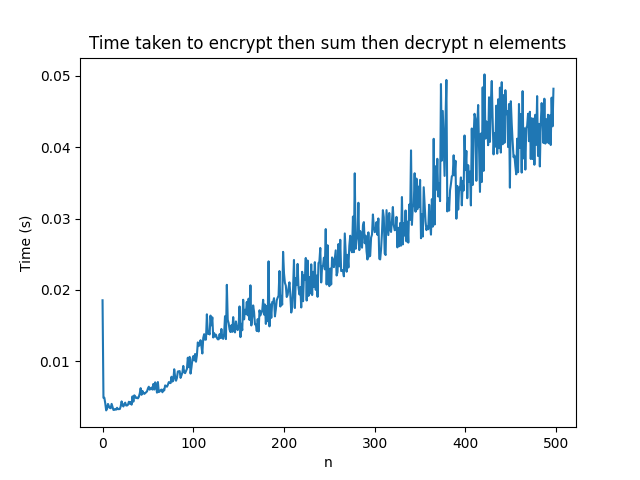
\includegraphics[width=0.5\linewidth]{Figure_1.png}
    \caption{Additions times}
    \label{fig:addition_time}
\end{figure}

\begin{figure}[!ht]
    \centering
    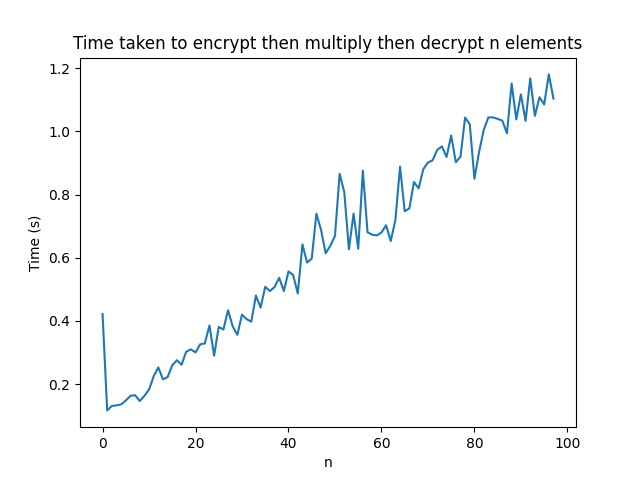
\includegraphics[width=0.5\linewidth]{Figure_2.png}
    \caption{Multiplication times}
    \label{fig:multiplication_time}
\end{figure}


\newpage

\section{Credits}

Marc Joye's guide \cite{joye_guide} helped us a lot to describe all the steps in TFHE, we relied on it a lot but tried to explain with our own words when possible. We tried to add a more intuitive idea at each step.



\begin{thebibliography}{9}

\bibitem{survey_marcolla}
Marcolla, Chiara; Sucasas, Victor; Manzano, Marc; Bassoli, Riccardo; Fitzek, Frank H.P.; Aaraj, Najwa (2022) \emph{Survey on Fully Homomorphic Encryption, Theory, and Applications}

\bibitem{FHEW}
Léo Ducas; Daniele Micciancio \emph{FHEW: Bootstrapping Homomorphic Encryption in less than a second}

\bibitem{joye_guide}
Marc Joye, Zama France; \emph{Guide to Fully Homomorphic Encryption over the [Discretized] Torus}

\bibitem{fhe_mathematicians}
Alice Silverberg; \emph{Fully Homomorphic Encryption For Mathematicians}

\bibitem{tfhe}
%TFHE: 
Ilaria Chillotti, Nicolas Gama, Mariya Georgieva and Malika Izabach; \emph{Fast Fully Homomorphic Encryption over the Torus}

\end{thebibliography}

\end{document}


